\chapter{Granger causality results on all patients}
\label{chapter:appendix-gc-results}
Here we report additional results for patients A, B and C for all combination of the epilepsy stages (preictal and interictal) and the frequency ranges (high frequency activities and infraslow activities). The bar diagram shows the total Granger causality, sink activity and source activity. The red circle represents seizure onset (SO) electrode and the blue circle represents contralateral electrode pair to the SO electrode. 
The result of patient C as a representative patient are included in the main part of this dissertation. 

%\section{High Frequency results for preictal state}

\begin{figure*}
\centerline{
	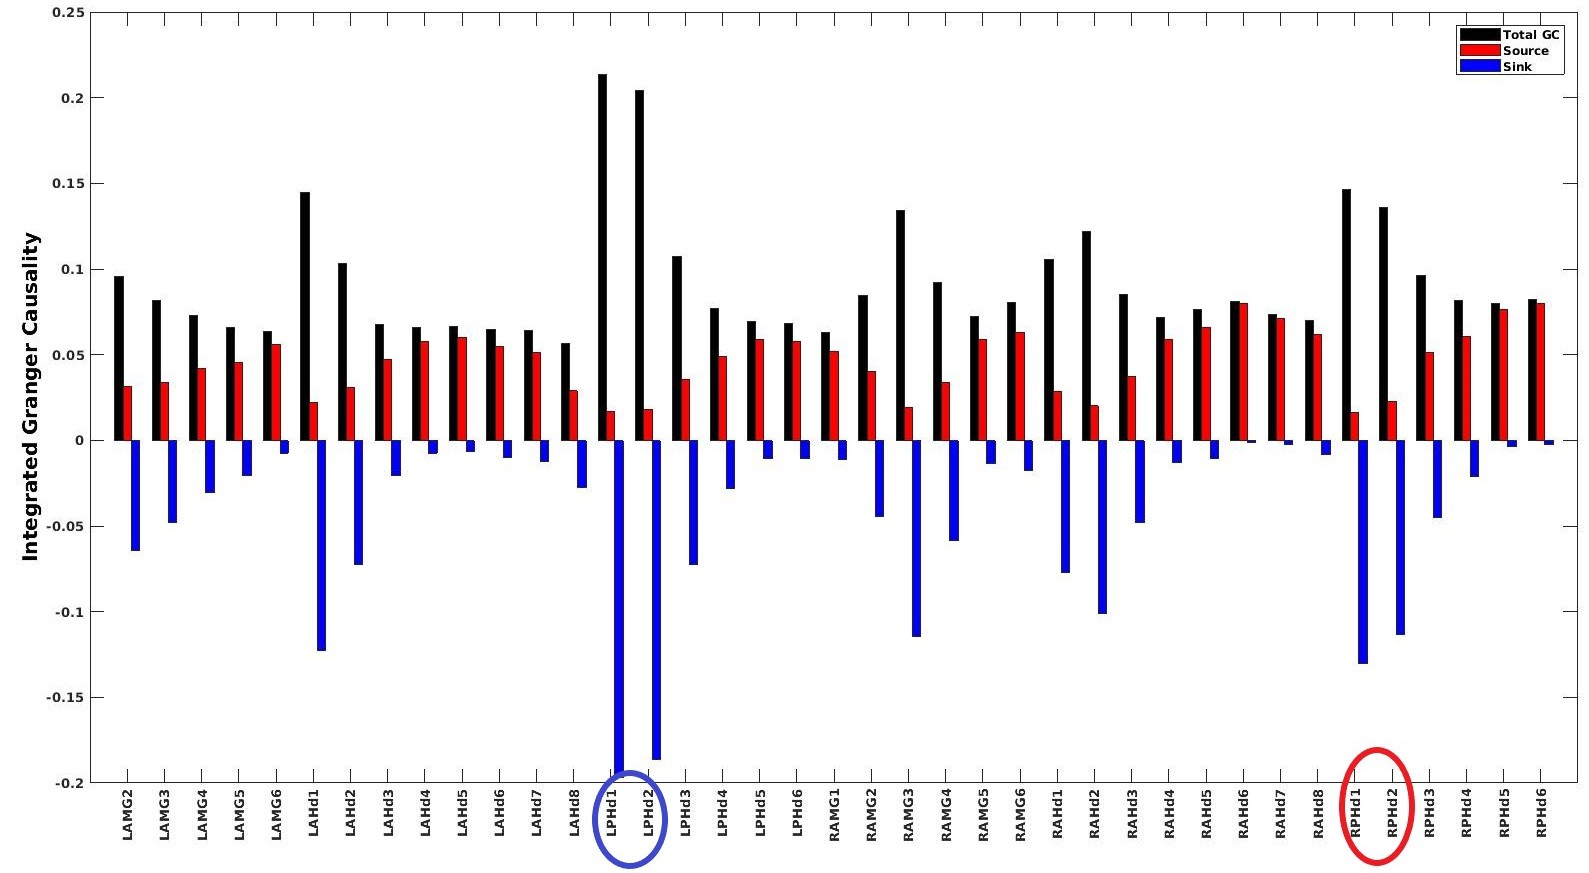
\includegraphics[height =3.5in]{Plots/Patient_A_preictal_high.jpg}
	}

	\caption{Patient A - Integrated Granger causality in the preictal state for high frequency activities}

	\label{fig:apdx_patient_a_preictal_high}
\end{figure*}


\begin{sidewaysfigure*}
\centerline{
	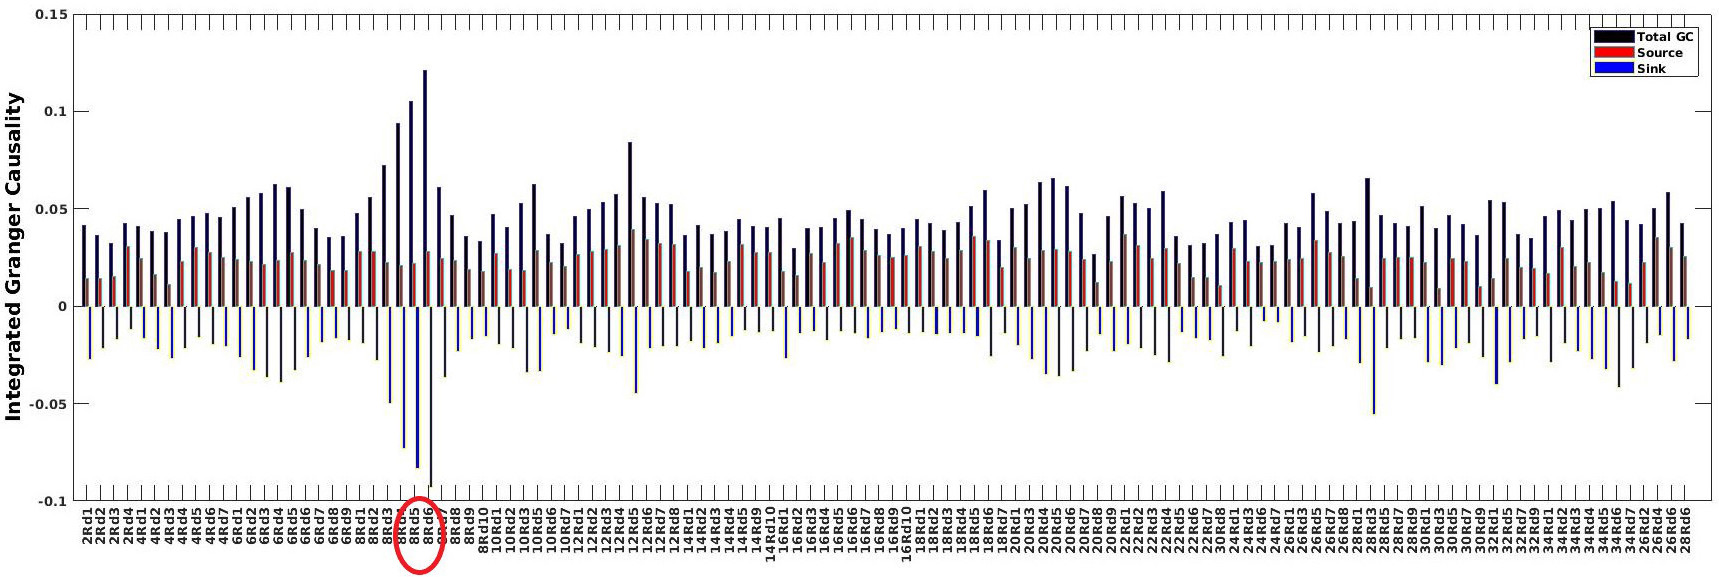
\includegraphics[height =2.8in]{Plots/Patient_B_preictal_high.jpg}
	}

	\caption{Patient B - Integrated Granger causality in the preictal state for high frequency activities}

	\label{fig:apdx_patient_b_preictal_high}
\end{sidewaysfigure*}

\begin{sidewaysfigure*}
\centerline{
	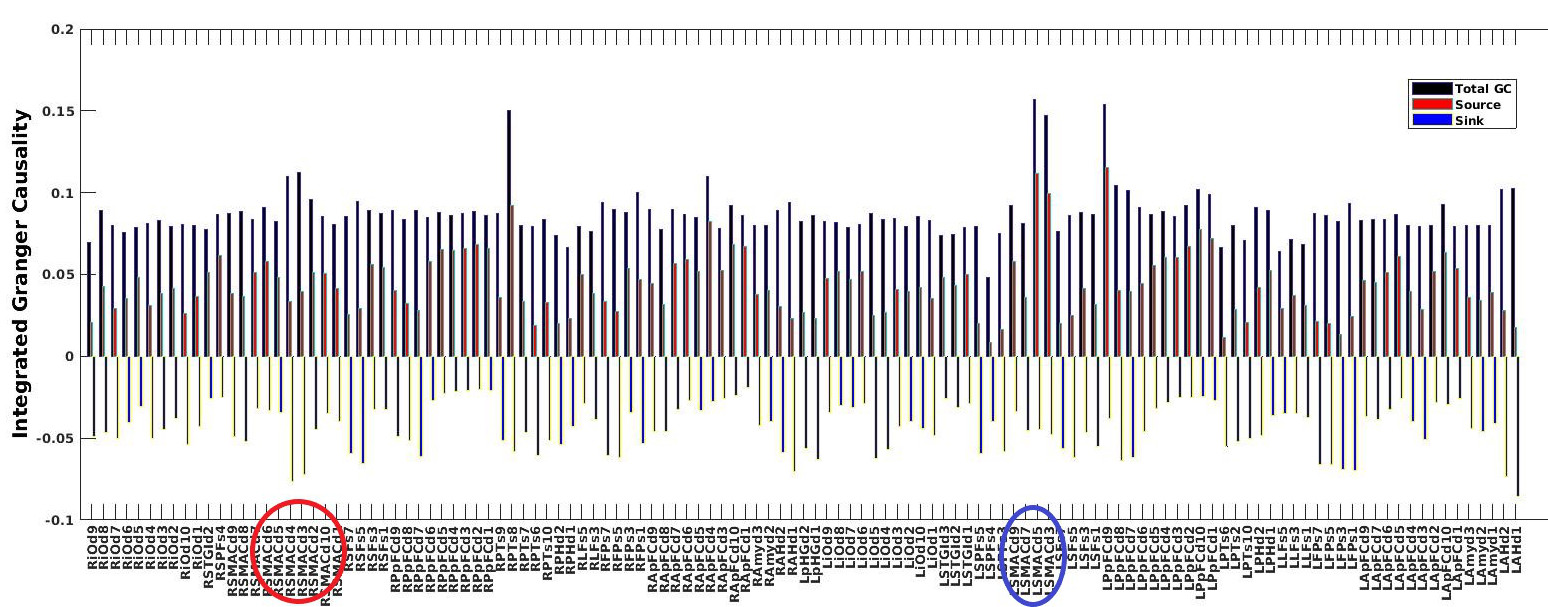
\includegraphics[height =3.2in]{Plots/Patient_C_preictal_high.jpg}
	}

	\caption{Patient C - Integrated Granger causality in the preictal state for high frequency activities}

	\label{fig:apdx_patient_c_preictal_high}
\end{sidewaysfigure*}


%\section{Granger causality on preictal infraslow}

\begin{figure*}
\centerline{
	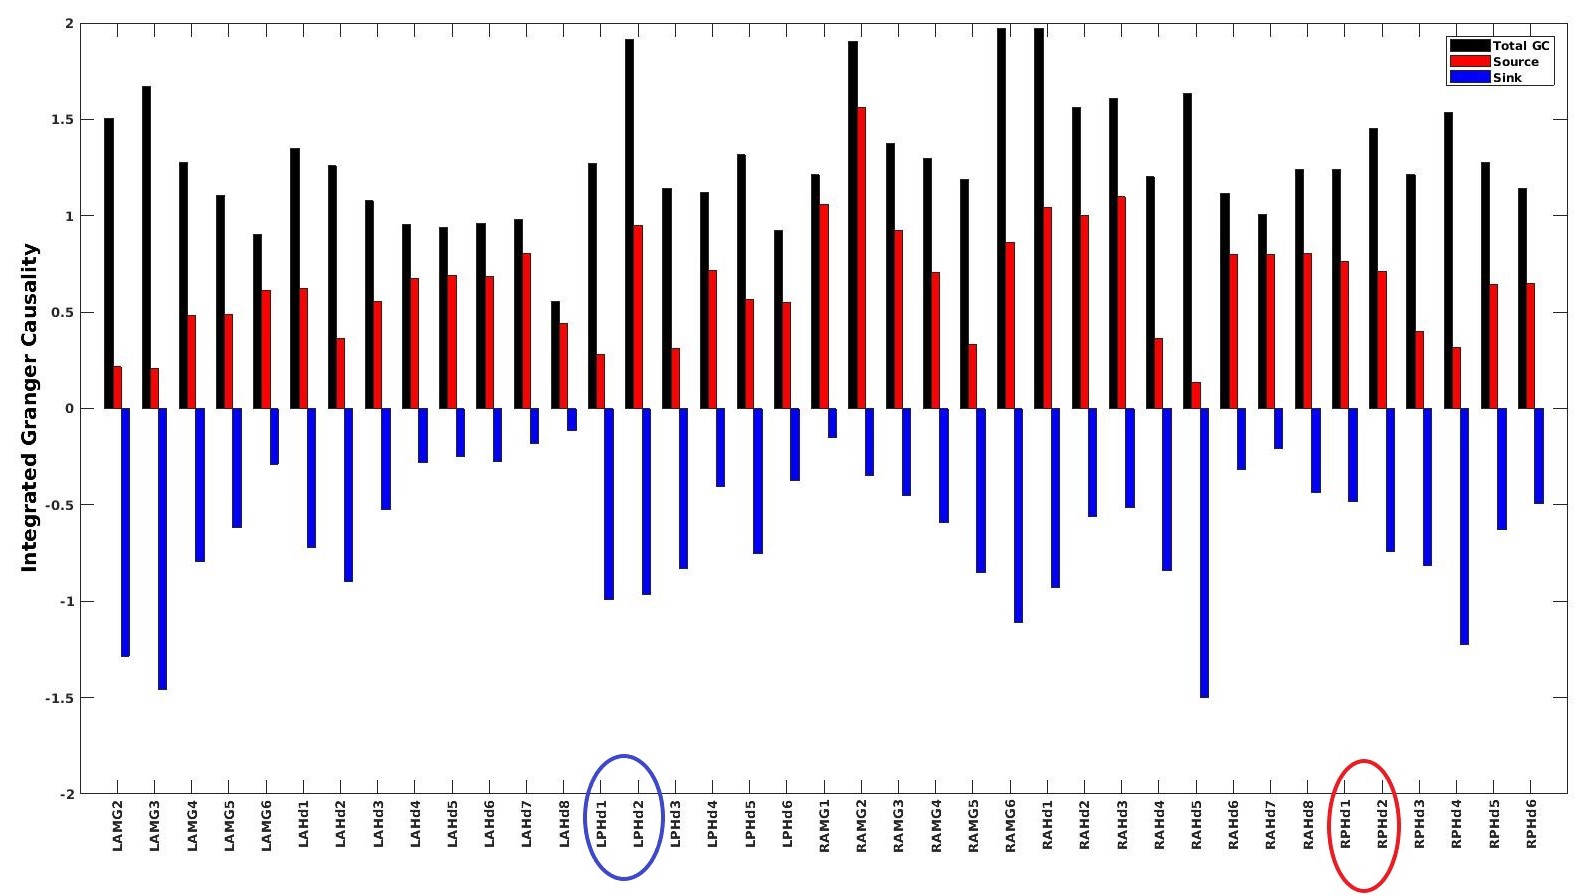
\includegraphics[height =3.5in]{Plots/Patient_A_preictal_low.jpg}
	}

	\caption{Patient A -  Integrated Granger causality in the preictal state for infraslow activities}

	\label{fig:apdx_patient_a_preictal_low}
\end{figure*}


\begin{sidewaysfigure*}
\centerline{
	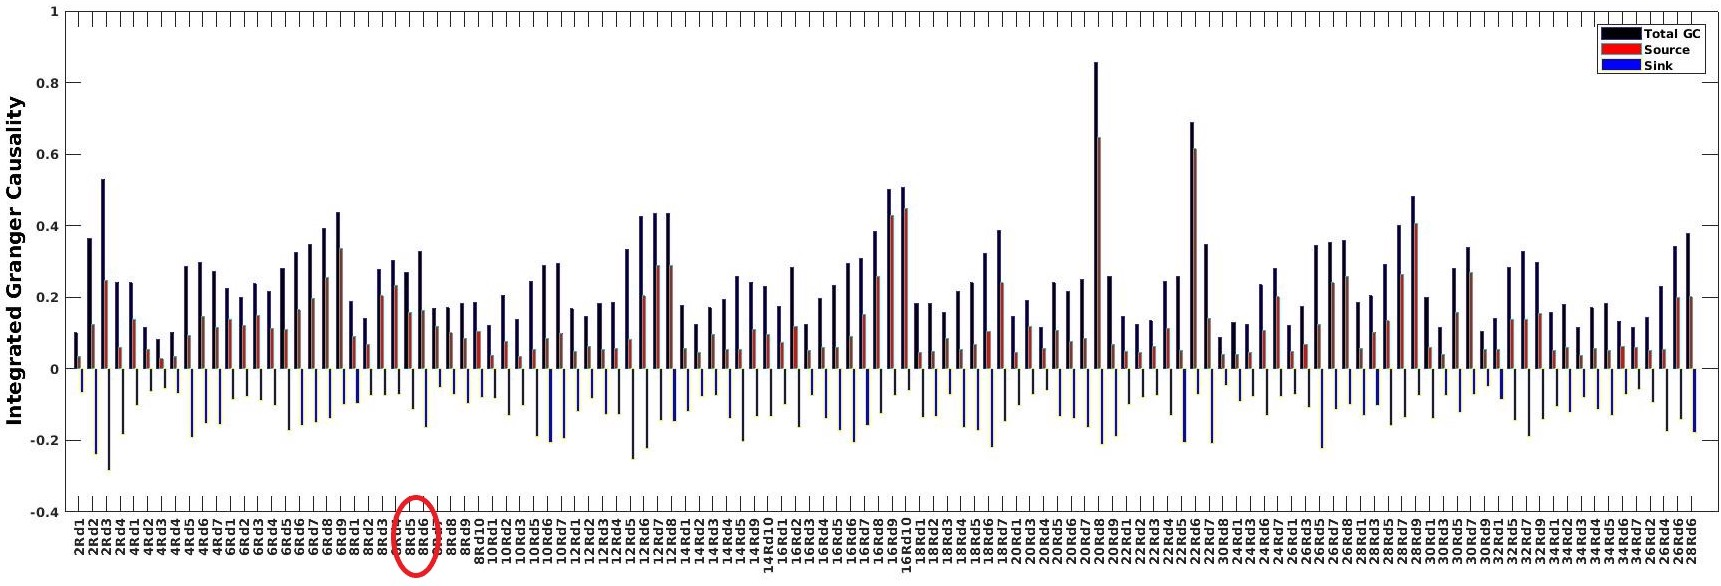
\includegraphics[height =2.8in]{Plots/Patient_B_preictal_low.jpg}
	}

	\caption{Patient B - Integrated Granger causality in the preictal state for infraslow activities}

	\label{fig:apdx_patient_b_preictal_low}
\end{sidewaysfigure*}


\begin{sidewaysfigure*}
\centerline{
	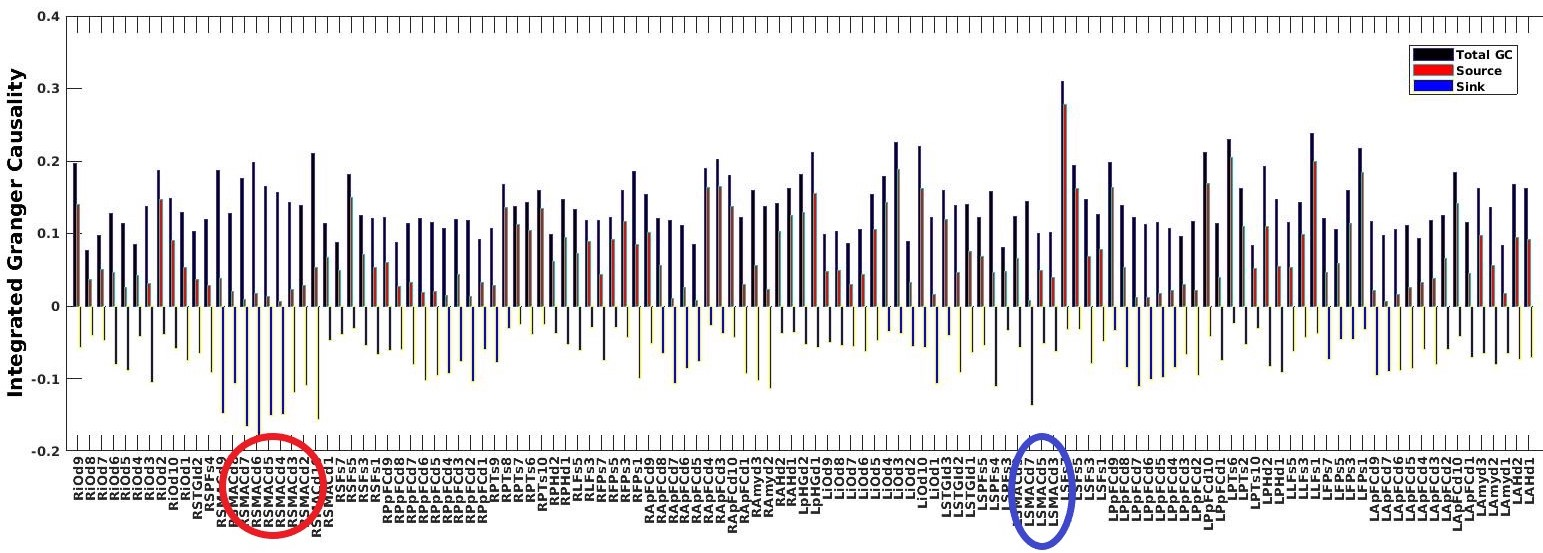
\includegraphics[height =3in]{Plots/Patient_C_preictal_low.jpg}
	}

	\caption{Patient C - Integrated Granger causality in the preictal state for infraslow activities}

	\label{fig:apdx_patient_c_preictal_low}
\end{sidewaysfigure*}


%\section{Granger causality on interictal high frequency}

\begin{figure*}
\centerline{
	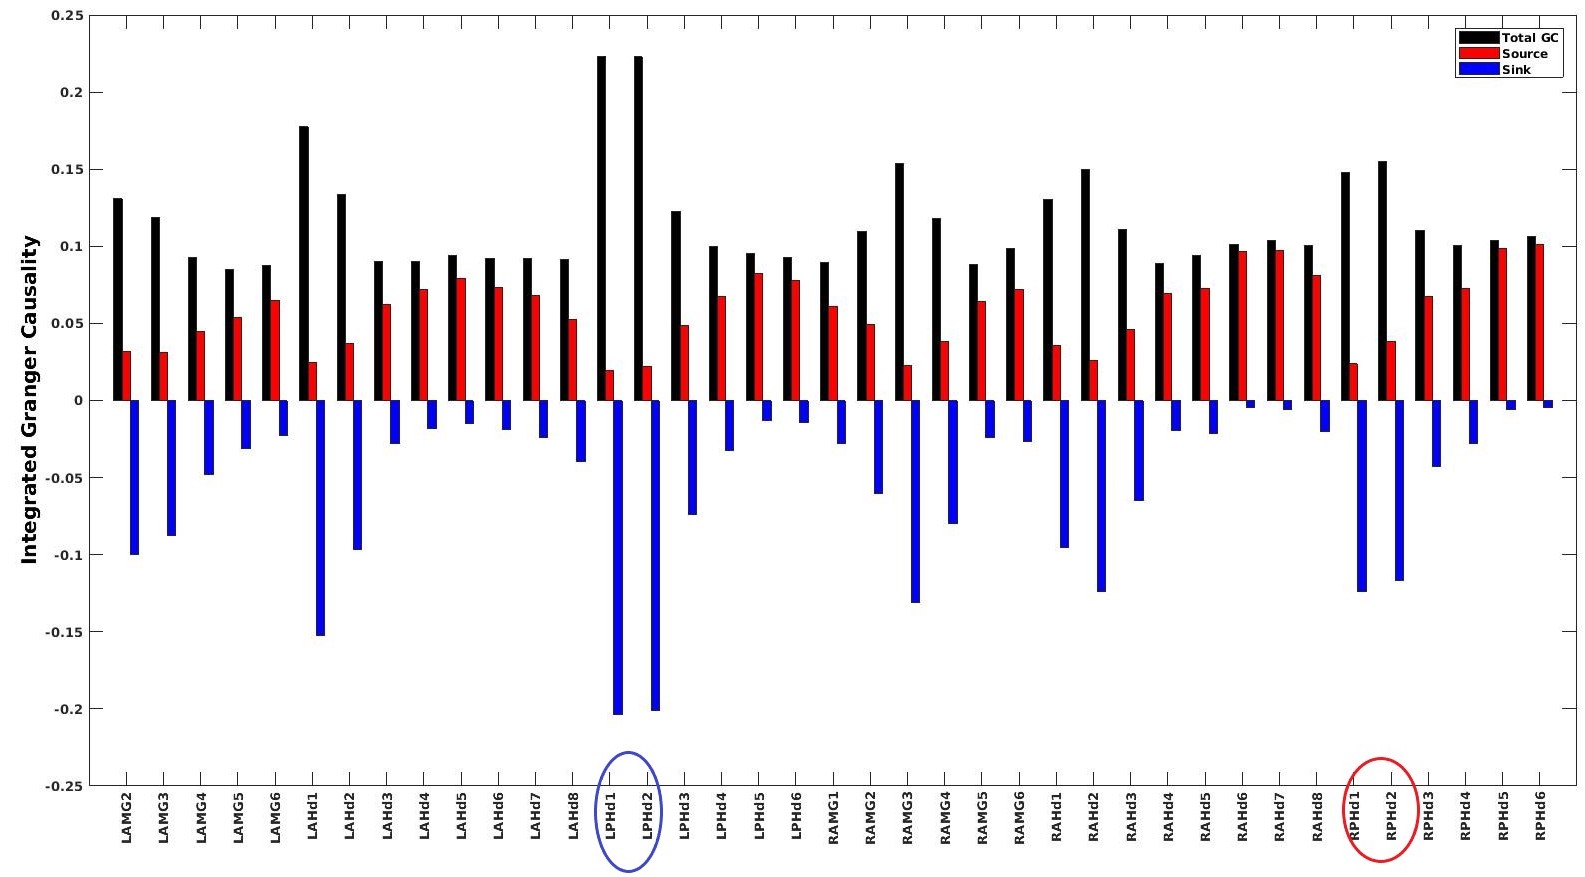
\includegraphics[height =3.5in]{Plots/Patient_A_interictal_high.jpg}
	}

	\caption{Patient A - Integrated Granger causality in the interictal state for high frequency activities}

	\label{fig:apdx_patient_a_interictal_high}
\end{figure*}


\begin{sidewaysfigure*}
\centerline{
	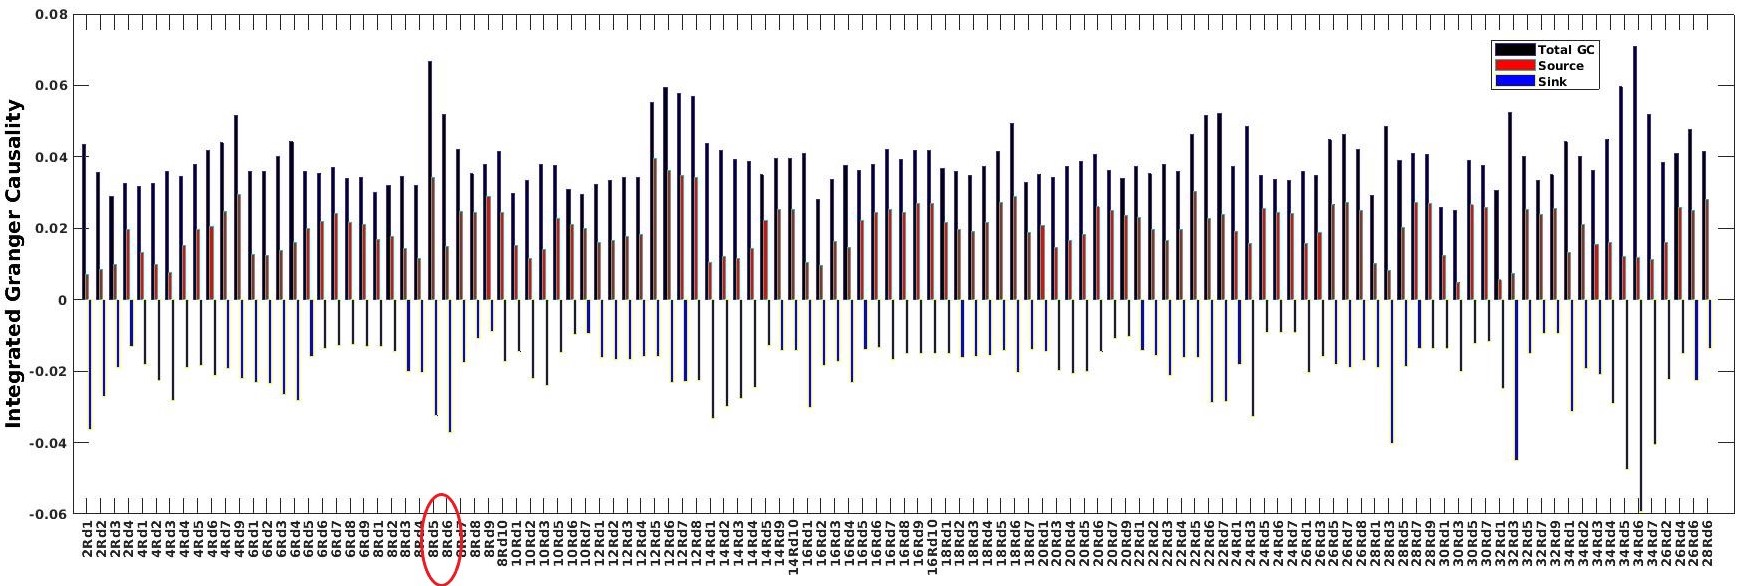
\includegraphics[height =2.8in]{Plots/Patient_B_interictal_high.jpg}
	}

	\caption{Patient B - Integrated Granger causality in the interictal state for high frequency activities}

	\label{fig:apdx_patient_b_interictal_high}
\end{sidewaysfigure*}

\begin{sidewaysfigure*}
\centerline{
	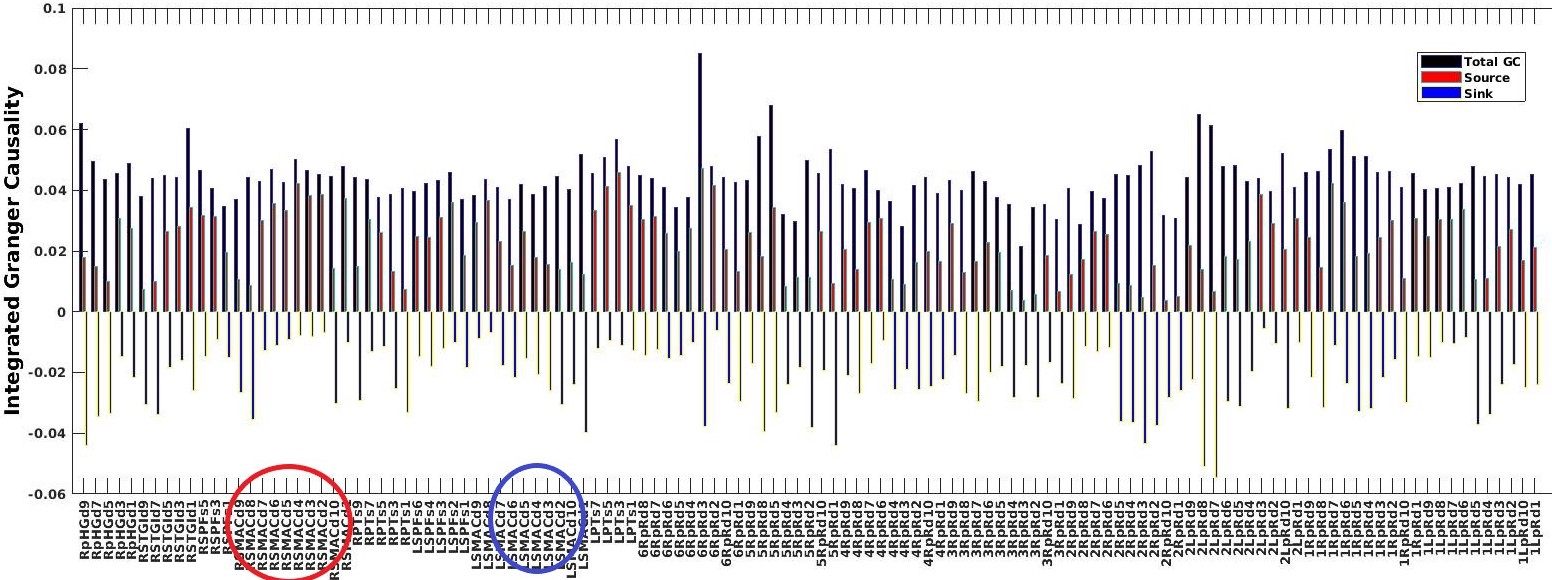
\includegraphics[height =3.1in]{Plots/Patient_C_interictal_high.jpg}
	}

	\caption{Patient C - Integrated Granger causality in the interictal state for high frequency activities}

	\label{fig:apdx_patient_c_interictal_high}
\end{sidewaysfigure*}



%\section{Granger causality on interictal infraslow}

\begin{figure*}
\centerline{
	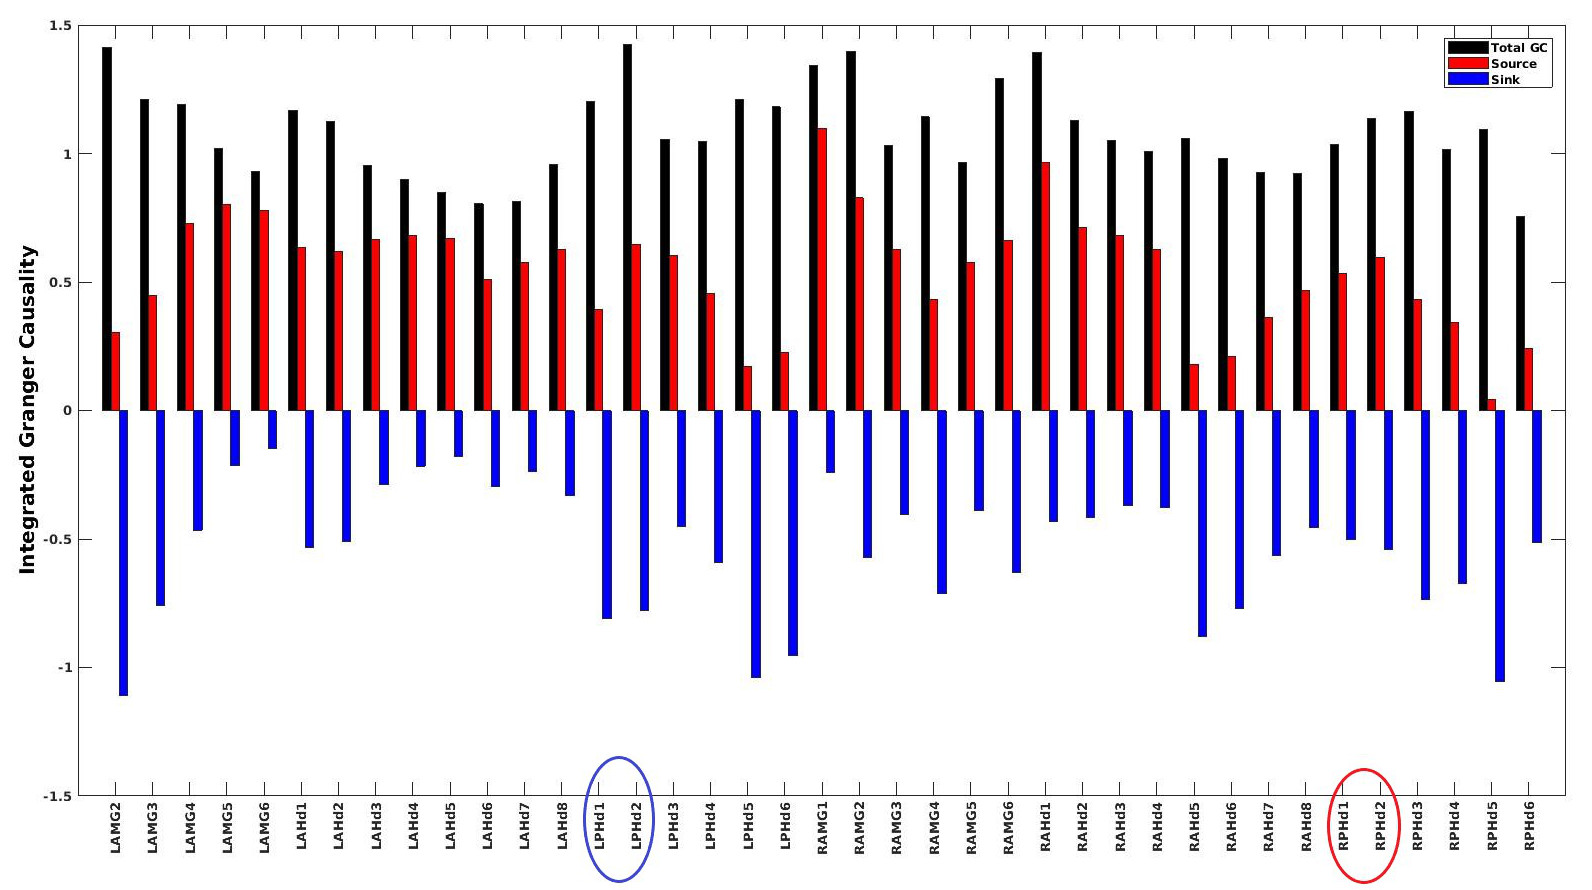
\includegraphics[height =3.5in]{Plots/Patient_A_interictal_low.jpg}
	}

	\caption{Patient A - Integrated Granger causality in the interictal state for infraslow activities}

	\label{fig:apdx_patient_a_interictal_low}
\end{figure*}

\begin{sidewaysfigure*}
\centerline{
	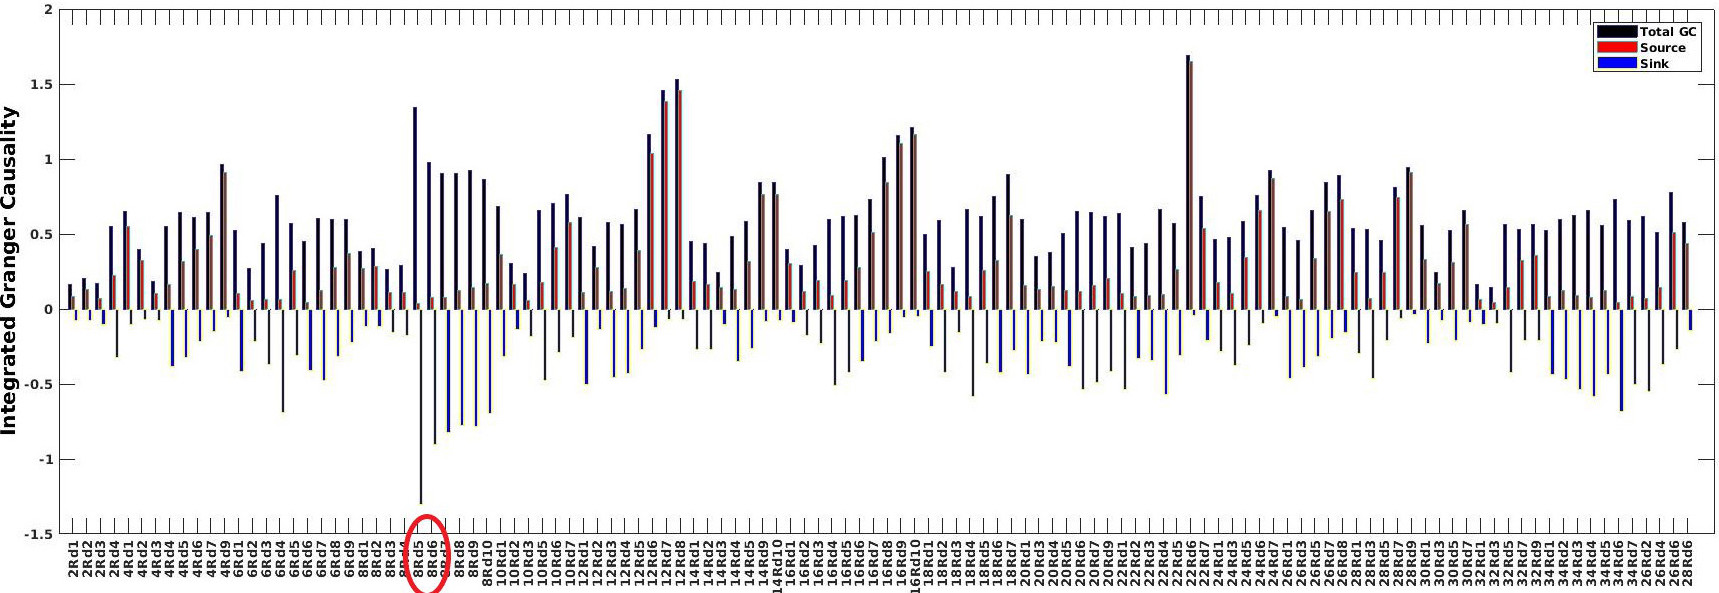
\includegraphics[height =2.8in]{Plots/Patient_B_interictal_low.jpg}
	}

	\caption{Patient B - Integrated Granger causality in the interictal state for infraslow activities}

	\label{fig:apdx_patient_b_interictal_low}
\end{sidewaysfigure*}


\begin{sidewaysfigure*}
\centerline{
	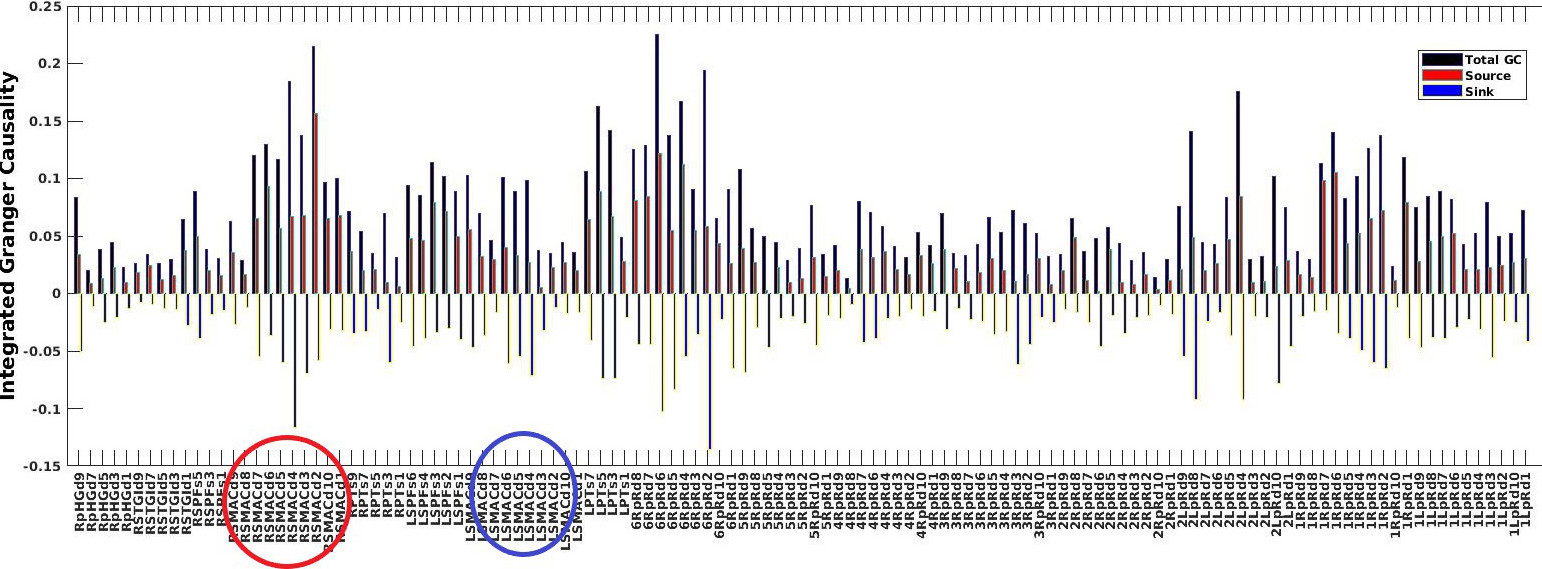
\includegraphics[height =3in]{Plots/Patient_C_interictal_low.jpg}
	}

	\caption{Patient C - Integrated Granger causality in the interictal state for infraslow activities}

	\label{fig:apdx_patient_c_interictal_low}
\end{sidewaysfigure*}